% -*- TeX -*- -*- UK -*- -*- BMR -*-
% ----------------------------------------------------------------
% Beamer presentation ************************************************
%
% Subhaneil Lahiri's template
%
% To compile:
%   Ctrl-Shift-P
%
% **** -----------------------------------------------------------
\documentclass{beamer}%[hyperref={backref=slide}]

\input{sl_slide_preamble.tex}
\input{sl_slide_graphics_preamble.tex}
\input{sl_definitions.tex}
\input{sl_slide_symbols.tex}
\graphicspath{{"Figures/"}}
%matrices
\newcommand{\I}{\mathbf{I}}
%vec of ones
%equilibrium distribution
\newcommand{\pr}{\mathbf{p}}
\newcommand{\eq}{\pr^\infty}
%other symbols
\newcommand{\w}{\mathbf{w}}
\newcommand{\W}{\mathbf{W}}
\newcommand{\frg}{\W^\mathrm{F}}
\newcommand{\M}{\mathbf{M}}
\newcommand{\F}{\boldsymbol{\Phi}}
\newcommand{\pot}{^{\text{pot}}}
\newcommand{\dep}{^{\text{dep}}}
\newcommand{\potdep}{^{\text{pot/dep}}}
\newcommand{\lmax}{_{\text{max}}}
\newcommand{\lmin}{_{\text{min}}}
%---------Title-----------------------------------------------------------

\title[Complex synapses]{A general theory of learning and memory with Complex Synapses}
%
\subtitle{\small{based on work with Surya Ganguli}
}
%
\author{Subhaneil Lahiri%\inst{1}
}
%
\institute[Stanford]{%
%\inst{1}
Stanford University, Applied Physics
}
%
%\slideCaption{}

%---------Beginning--------------------------------------------------------

\begin{document}

%-------------Slide--------------------------------------------------------

\begin{frame}
%
 \titlepage
%
\end{frame}

%-------------Slide--------------------------------------------------------

\begin{frame}{Introduction}
%
 We often model synaptic plasticity as the change of a single number (synaptic weight).
 \note[item]{amplitude of psp.}
 In reality, there is a complex dynamical system inside a synapse.

 \vp Semi-realistic models of synaptic memory have terrible storage without synaptic complexity.
 \note[item]{finite number of values.}

 \vp We will study the entire space of a broad class of models of complex synapses to find upper bounds on their performance.

%
\end{frame}

%-------------Slide--------------------------------------------------------

\begin{frame}{Outline}
%
 \tableofcontents[hideallsubsections]
 \note[item]{review terrible properties of simple synapses.}
 \note[item]{mathematical formalism of model, quantify performance (memory decay over time)}
 \note[item]{upper bounds on single numbers that describe performance at all times}
 \note[item]{upper bounds at finite times}
%
\end{frame}

%-------------Section--------------------------------------------------------

\section{Why complex synapses?}

%-------------Slide--------------------------------------------------------

\begin{frame}{Complex synapse}
%
 \begin{center}
 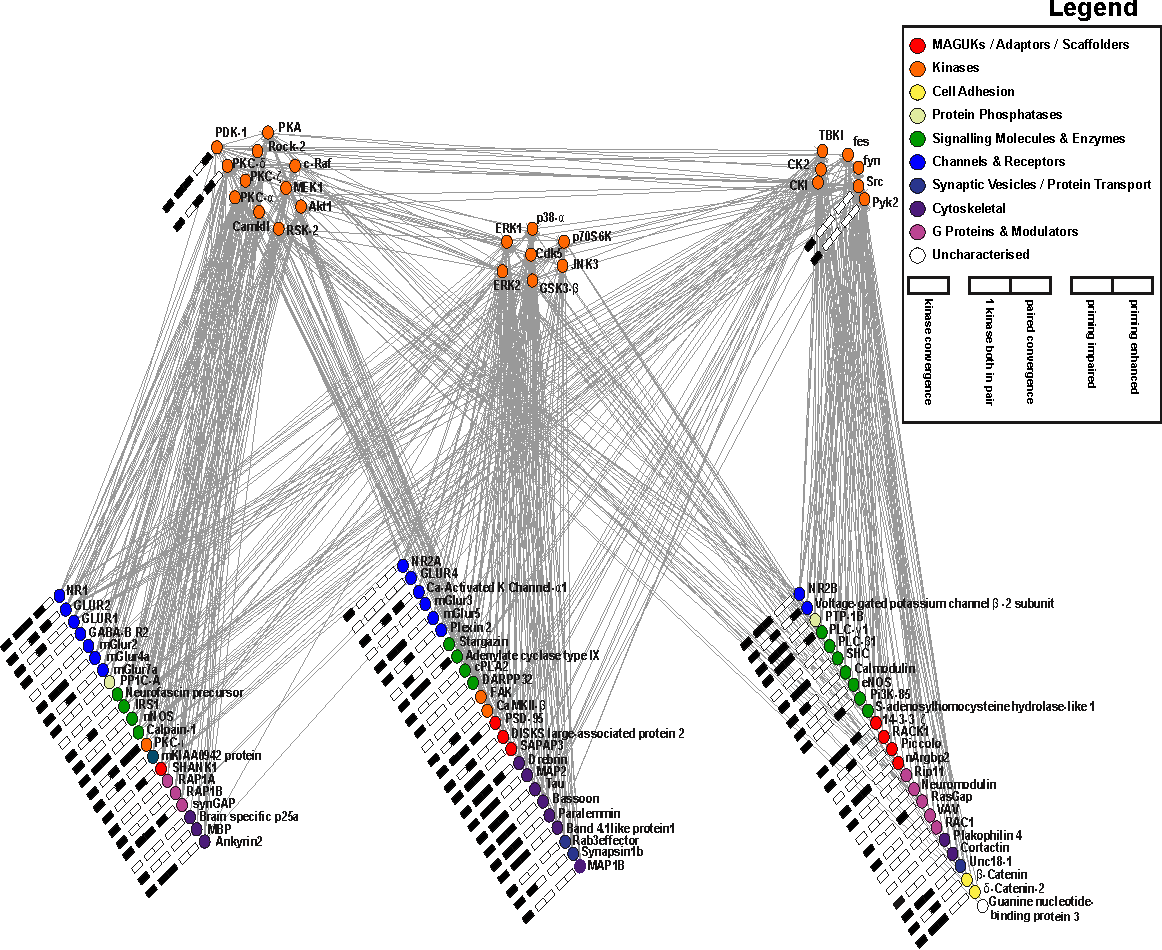
\includegraphics[height=6cm]{2000102CobaFig4.pdf}\citerrr{Coba2009phosphorylation}
 \end{center}
 There is a complex, dynamical molecular network underlying synaptic plasticity.
 \note[item]{Does this matter?}
 \note[item]{Could just be the machinery for changing synaptic weight}
%
\end{frame}

%-------------Slide--------------------------------------------------------

\begin{frame}{Storage capacity of synaptic memory}
%
  A classical perceptron (used as a recognition memory device) has a capacity $\propto N$, the number of synapses.

 \vp Requires synapses' dynamic range also $\propto N$.

 \vp If we restrict synaptic weight to a fixed, finite set of values,\\
 \hp $\implies$ tradeoff between learning and forgetting:\\
 \hp new memories overwriting old.

 \vp If we wish to store new memories rapidly, memory capacity  $\sim\CO(\log N)$.
 \\ \citerr{amit1992constraints,amit1994learning}

 \vp To circumvent this tradeoff, need to go beyond model of a synapse as a single number.
%
\end{frame}

%-------------Section--------------------------------------------------------

\section{Modelling synaptic complexity}

%-------------Slide--------------------------------------------------------

\begin{frame}{Complex synapses}
%
  \aligntop{\includegraphics[width=5cm]{synapse.svg}}
  \hp\aligntop{\includegraphics[width=2cm]{pot.svg}}
  \hp\aligntop{\includegraphics[width=2cm]{dep.svg}}
%
\end{frame}

%-------------Slide--------------------------------------------------------

\begin{frame}{Simplifying assumptions}
%
\begin{itemize}
  \item There are $N$ identical synapses with $M$ internal functional states.
  \item States of different synapses are independent of each other.
  \item Which synapses eligible for plasticity chosen randomly.
  \item Potentiating/depressing plasticity events $\sim$ Poisson processes with rates $rf\potdep$, where $f\pot+f\dep=1$.
      \note{In other words, $r$ is the total rate of plasticity events per synapse and $f\potdep$ are the fraction of these events that are potentiating/depressing.}
  \item Potentiation and depression are described by Markov processes with transition probabilities $\M\potdep$.
  \item Synaptic weights of the internal states are given by vector $\w$.\\ Can only take values $\pm1$.
\end{itemize}
%
\end{frame}


%-------------Section--------------------------------------------------------

\section{Upper bounds}

%-------------Slide--------------------------------------------------------


%-------------Section--------------------------------------------------------

\section{Envelope memory curve}

%-------------Slide--------------------------------------------------------






%-------------Slide--------------------------------------------------------
%
%% Press Ctrl-D to insert a new slide
%
%
%-------------Slide--------------------------------------------------------

\begin{frame}{Acknowledgements}
%
 Thanks to:
 \begin{itemize}
   \item Surya Ganguli
   \item Stefano Fusi
   \item Marcus Benna
 \end{itemize}
 \note[item]{Last slide!}
%
\end{frame}

%-------------Slide--------------------------------------------------------

\begin{frame}[allowframebreaks]{References}
%

 {\small
 \bibliographystyle{unsrt_slides}
 \bibliography{maths,neuro}
 }
%
\end{frame}


%-----End----------------------------------------------------------------

\end{document}
